% Bitemporal supersession: a dirty write-back closes the prior observation's valid_to
% and opens a fresh valid_from row — never in-place — so older trace positions still
% read older bytes. Evicted working-set rows are retained (state='evicted'), not deleted.
\documentclass[border=8pt]{standalone}
\usepackage{tikz}
\usetikzlibrary{arrows.meta}
\usepackage{xcolor}
\definecolor{oldc}{HTML}{6B7280}
\definecolor{newc}{HTML}{16A34A}
\definecolor{axisc}{HTML}{475569}
\begin{document}
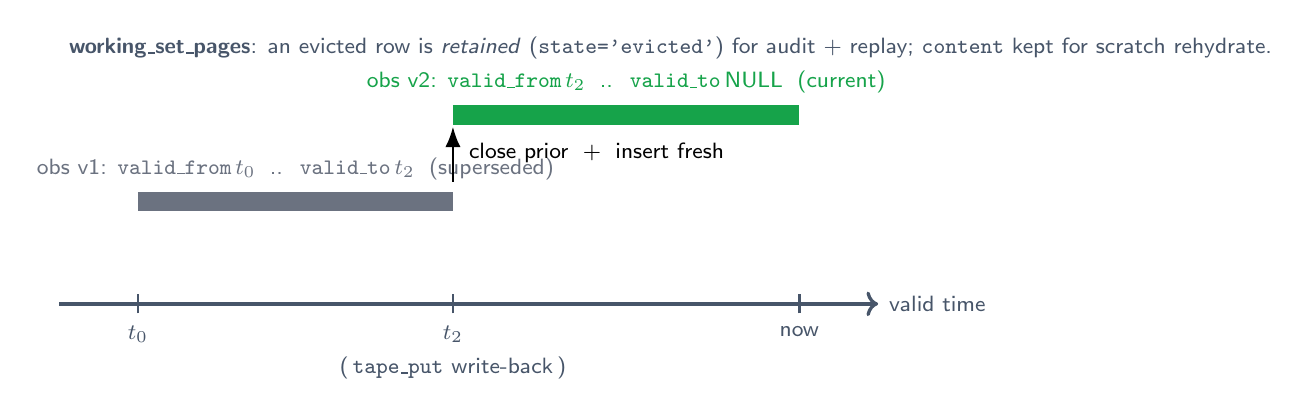
\begin{tikzpicture}[font=\sffamily\footnotesize, x=1cm, y=1cm]
  % time axis
  \draw[->, axisc, very thick] (0,0) -- (10.4,0) node[right]{valid time};
  \foreach \x/\l in {1/{$t_0$}, 5/{$t_2$}, 9.4/{now}} {
    \draw[axisc, thick] (\x,-0.12) -- (\x,0.12);
    \node[below, axisc] at (\x,-0.16) {\l};
  }
  \node[below, axisc] at (5,-0.55) {(\,\texttt{tape\_put} write-back\,)};

  % v1 interval (superseded)
  \draw[oldc, line width=7pt] (1,1.3) -- (5,1.3);
  \node[oldc, above] at (3.0,1.45) {obs v1: \texttt{valid\_from}\,$t_0$ \;..\; \texttt{valid\_to}\,$t_2$ \;(superseded)};
  % v2 interval (current)
  \draw[newc, line width=7pt] (5,2.4) -- (9.4,2.4);
  \node[newc, above] at (7.2,2.55) {obs v2: \texttt{valid\_from}\,$t_2$ \;..\; \texttt{valid\_to}\,NULL \;(current)};
  % supersede arrow
  \draw[-{Latex[length=2.6mm]}, thick] (5,1.55) -- (5,2.25);
  \node[right] at (5.08,1.92) {close prior \;+\; insert fresh};

  \node[align=left, anchor=west, axisc] at (0,3.25)
    {\textbf{working\_set\_pages}: an evicted row is \emph{retained} (\texttt{state='evicted'}) for audit + replay; \texttt{content} kept for scratch rehydrate.};
\end{tikzpicture}
\end{document}
